\documentclass[12pt]{beamer}

\hypersetup{colorlinks=true,linkcolor=red}
\usetheme{default}
\usecolortheme{albatross}

\usepackage[utf8]{inputenc}
\usepackage[russian,english]{babel}
\usepackage[T2A]{fontenc}
\usepackage{hyperref}
\usepackage[final]{listings}
\usepackage{breakurl}
\usepackage{cite}
\usepackage{perpage}

\graphicspath{{img/}}

\def\Url\Breaks{\do\/\do-}
\lstset{
  frame=single,
  breaklines=true,
  basicstyle=\tiny,
  postbreak=\raisebox{0ex}{\ensuremath{\hookrightarrow\space}},
  numbers=left
}

\lstdefinestyle{base}{
  frame=single,
  breaklines=true,
  basicstyle=\tiny,
  postbreak=\raisebox{0ex}{\ensuremath{\hookrightarrow\space}},
  moredelim=[is][\color{red}]{@}{@},
  numbers=left
}

\MakePerPage{footnote}

\title{Operating Systems}
\subtitle{Permanent Storage}
\author{Me}
\date{\today}

\begin{document}
  \begin{frame}
    \titlepage
  \end{frame}

  \begin{frame}
\frametitle{Блочные устройства}
\begin{itemize}
  \item Блочные устройства - устройсва с поблочным доступом
  \begin{itemize}
    \item общение с устройством идет порциями кратными некоторому фиксированному
    размеру - сектору
    \item типичный размер сектора - 512 байт;
    \item внутри устройство может работать с блоками произвольного размера, но
    интерфейс зачастую в 512 байтных блоках.
  \end{itemize}
  \item Типичные примеры блочных устройств:
  \begin{itemize}
    \item жесткие диски (HDD) и твердотельные накопители (SSD);
    \item оптические диски (CD, DVD, etc);
    \item даже USB Flash накопители...
  \end{itemize}
\end{itemize}
\end{frame}

  \begin{frame}
\frametitle{Механические диски (HDD)}
\begin{columns}
  \begin{column}{.6\linewidth}
    \begin{center}
      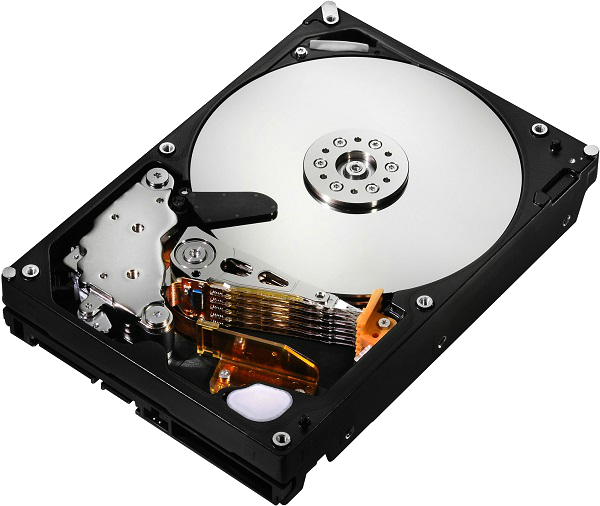
\includegraphics[width=.9\linewidth]{hdd.png}
    \end{center}
  \end{column}
  \begin{column}{.55\linewidth}
    Три основных части:
    \begin{itemize}
      \item вращающиеся диски (platters);
      \item подвижная рука (arm);
      \item читающие/пишушие головы (heads);
    \end{itemize}
  \end{column}
\end{columns}
\end{frame}

\begin{frame}
\frametitle{Скорость HDD}
\begin{itemize}
  \item Скорость вращения дисков HDD:
  \begin{itemize}
    \item при скорости 7200 оборотов в минуту - один оборот 8-9 мс;
    \item чтобы записать/прочитать данные нужно поставить голову над/под нужным
    цилиндром и подождать, пока нужное место диска "доедет" до головы.
  \end{itemize}
  \item Скорость позиционирования читающей/пишушей головы:
  \begin{itemize}
    \item время определяется опять же миллисекундами.
  \end{itemize}
  \item Скорость работы диска доминируется поиском:
  \begin{itemize}
    \item скорость вращения диска + позиционирование головы;
    \item random IO гораздо медленнее sequential IO.
  \end{itemize}
\end{itemize}
\end{frame}

\begin{frame}
\frametitle{Скорость HDD}
\begin{center}
  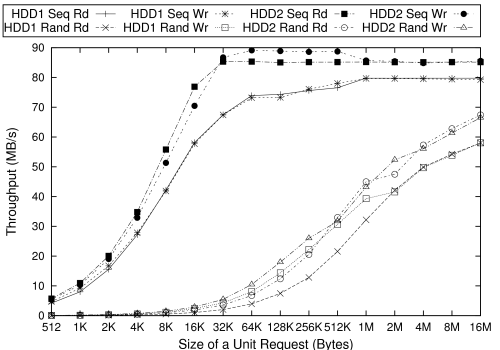
\includegraphics[width=.8\linewidth]{hdd_perf.png}
\end{center}
\end{frame}

  \begin{frame}
\frametitle{Твердотельные накопители (SSD)}
\end{frame}


  \begin{frame}
  \begin{center}
  \Huge Q\&A
  \end{center}
  \end{frame}
\end{document}
